\documentclass[10pt]{article}
\usepackage[margin=0.7in]{geometry}
\usepackage[T1]{fontenc}
\usepackage{lmodern,graphicx,booktabs,array,hyperref,fancyhdr}
\hypersetup{colorlinks=true,urlcolor=blue}
\pagestyle{fancy}\fancyhf{}\lhead{Classical prime-field ECDLP counter audit}\rhead{23 November 2026}\cfoot{Unsigned producer claims --- \thepage}
\setlength{\headheight}{14pt}\setlength{\parindent}{0pt}\setlength{\parskip}{5pt}
\begin{document}
{\Large\bfseries Checked scalar precision bound and controls}

The shared integer model has kernel-checked increment and conditional precision
bounds, with one valid scalar instance and six premise-deletion counterexamples.
The native PCC Lean verifier and seven-control proof gate pass. The local
verifier passes; claim \texttt{PCC-20261123-75fa8c} remains unsigned and
unverified in ledger standing.

Here $M$ counts network edges, $P$ is precision in bits, $u$ is a scale,
$a=A+2u$, $i<u$, $D=2^{a-i}$ and $h=\lceil3M/u\rceil$.
The source precision expression is
\[
P_{\rm child}=P+8hD+8M(a+1).
\]
The shared theorem establishes the exact multiplied-through bound
\[
u P_{\rm child}\le34MD
\]
assuming all six premises:
\[
u\le M,\quad i<u,\quad s\le Mq,\quad P\le cs2^A,
\]
\[
cqu\le2^{u+1},\qquad8u(A+2u+1)\le2^{A+u+1}.
\]
The coefficient $c$ is a parameter. The proof allocates $MD$, $32MD$ and
$MD$ to inherited precision, node loss and evaluation loss after multiplying
by $u$. A second theorem bounds one increment by $40M2^a$ for positive
$u\le M$. These are integer resource inequalities, not operation counts or
runtime ratios.

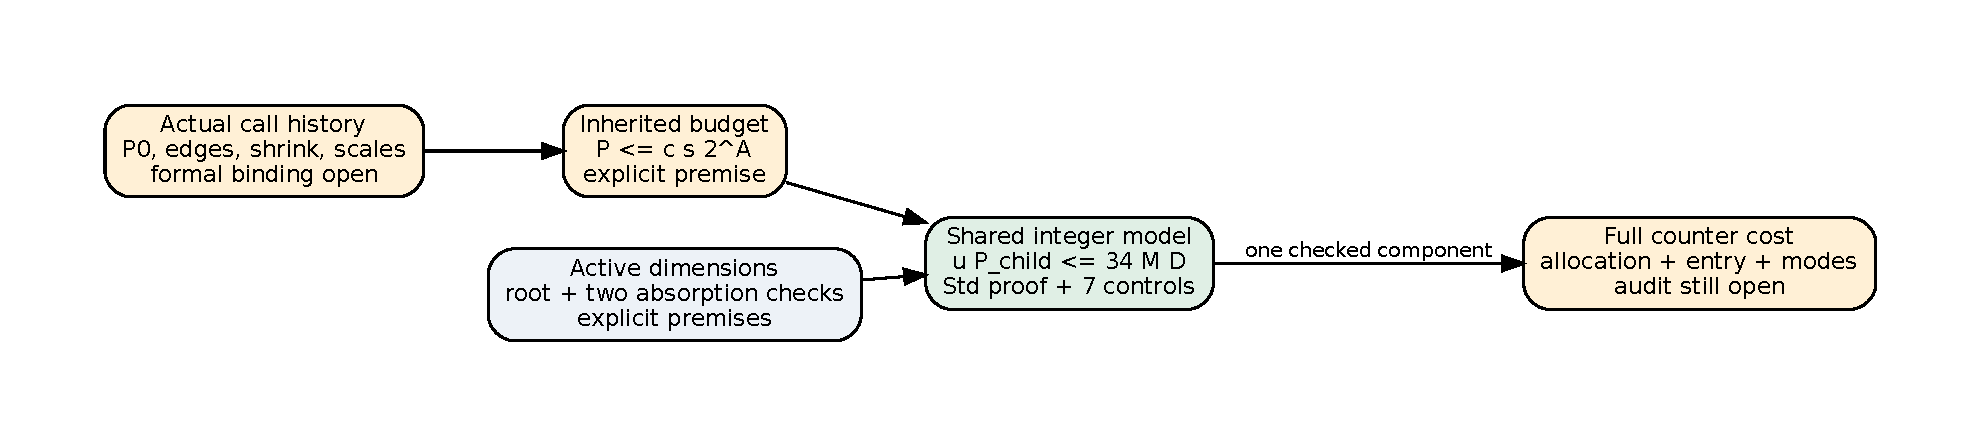
\includegraphics[width=\linewidth]{precision-map.pdf}

\textbf{Source.} Appendix D.11, openai/math revision42907c9e, TeX
blob51ba54ef. Native expression: crypto main816f9c3a,
\path{crates/hashed-ecdl-tensor/src/contraction/recursive.rs}.
Shared model: crypto-lean PR35, commit3e47fb77. The native qualification
copy matches upstream source byte for byte. This is a finite conditional
refinement of the existing argument, with no novelty assessment.

\textbf{Scope.} The theorem uses exact Nat arithmetic. It does not model
Rust overflow/error behavior, prove the inherited budget for every path,
admit a recursive graph, price the full counter, or establish an ECDLP cost
improvement. The user's objective remains classical only, with Amazon S3 storage excluded.

\newpage
{\Large\bfseries Controls, fidelity and remaining obligations}

\begin{tabular}{@{}p{0.30\linewidth}p{0.65\linewidth}@{}}\toprule
Control & Checked statement \\\midrule
Positive scalar & $P=64,M=128,u=16,A=0,i=15,s=128,q=8,c=81$ meets all premises and the bound.\\
Six deletion controls & Each retains the other five hypotheses, drops one, and proves a numerical counterexample to the resulting uniform statement.\\
Axiom inspection & Three shared statements and seven controls; only \texttt{propext}/\texttt{Quot.sound} in inequalities, none in the six finite counterexamples.\\
Repository gates & Native local theorem verifier passes; controls gate reports seven theorems and zero trusted-native entries.\\\bottomrule
\end{tabular}

Deleting a premise can admit a counterexample without making every sufficient
condition pointwise necessary. These scalar instances are not allocated public
recursive graphs or new solver executions. The controls observation claim
\texttt{PCC-20261123-a53245} is unsigned.

\textbf{Fidelity.} On active inputs, the native packet shift equals
$2^{a-i}$, and exact natural ceiling matches \texttt{div\_ceil} on successful
checked operations. The shared library owns the reusable model before the
study's numerical instances. No dependency, toolchain, proof-gate code or trust
list changes. This module imports only Std on pinned Lean4.35.0; the separate
Mathlib assembly probe does not enter its import closure.

The separate same-team reviewer found no blocking scalar algebra, source or
control issue and matched the shared commit, source blob and exact declaration
hash. Its local review is unsigned and distinct from execution attestation;
native committed-artifact binding follows separately.

\textbf{History remains open.} The written coefficient81 requires both
$P_0\le s$ and $M_0\le s$, plus $1/8$ path shrinkage. The native nonempty
normalization $s=2E,P_0=E+1$ supplies that initial scale. The manuscript's
general $P_0\le Cs$ alone does not fix81. A complete formal history binding,
source-guard absorption and packet/mode, creation-precision, rational-width,
allocation and entry bit-work proofs remain. The frozen84-case comparison
and optimized baseline reconciliation are separate open solver work.

\textbf{Failure and resource record.} Root-path, managed import-loader-cap,
typing/import and Std projection errors are retained. Gates06/07 reached the
unchanged whole-cgroup stop and returned no verdict. Gate09 passes after
lossless compaction of generated external dependency caches. Every archived
cache byte was compared and rehashed before compacting its duplicate
uncompressed copy; owned research, proof checkpoints and native executables
remain intact. Restore the documented caches before Mathlib builds.

All checks used the existing local machine, one Lean worker, a600-second phase
cap and15,032,385,536-byte whole-cgroup stop, with no new capacity, added spend
or S3. No theorem premise or gate was weakened to obtain the pass.

\textbf{Evidence.} The README links the source, proof/instance map, raw
successes and failures, local verdict and immutable scalar review. Shared
Mathlib-library/current-root CI remains separate from this focused component.

\small \url{https://github.com/isogeny-labs/crypto/pull/4996}\quad
\url{https://github.com/aburan28/crypto-lean/pull/35}
\end{document}
